\documentclass[11pt,a4paper]{article}
\usepackage{tikz,tkz-graph,amssymb,amsmath,amsthm,multirow,color,xcolor,cancel,bbm}
\usepackage[textheight=25cm,textwidth=16cm]{geometry}

\newtheorem{lemma}{Lemma}
\newtheorem{corollary}{Corollary}
\newtheorem{question}{Question}
\newtheorem{remark}{Remark}
\newtheorem{theorem}{Theorem}
\newtheorem{example}{Example}

\def\cst{\mathrm{cst}}
\def\B{\{0,1\}}
\def\In{\mathrm{In}}
\def\e{\epsilon}

\title{Fixed points and connections between positive and negative cycles in Boolean networks}

\author{
Adrien Richard\footnote{Laboratoire I3S, CNRS, Universit\'e C\^ote d'Azur \& Universit\'e Nice Sophia Antipolis, France.
\tt{richard@unice.fr}}
}

\date{November 28, 2016; Revised November 14, 2017}

\begin{document}

\maketitle

\begin{abstract} 
We are interested in the relationships between the number fixed points in a Boolean network  and its interaction graph, which is the arc-signed digraph  on  that describes the positive and negative influences between the components of the network. A fundamental theorem of Aracena says that if  has no positive (resp. negative) cycle, then  has at most (resp. at least) one fixed point; the sign of a cycle being the product of the signs of its arcs. In this note, we generalize this result by taking into account the influence of connections between positive and negative cycles. In particular, we prove that if every positive (resp. negative) cycle of  has an arc  such that  has a non-trivial initial strongly connected component containing the terminal vertex of  and only negative (resp. positive) cycles, then  has at most (resp. at least) one fixed point. This is, up to our knowledge, the first generalization of Aracena's theorem where the conditions are expressed with  only. 




\medskip\noindent
{\bf Keywords:} Boolean network, fixed point, interaction graph, positive cycle, negative cycle. 
\end{abstract}

\section{Introduction}


A {\em Boolean network} with  components is a discrete dynamical system usually defined by a global transition function

Boolean networks have many applications. In particular, since the seminal papers of McCulloch and Pitts \cite{MP43}, Hopfield \cite{H82}, Kauffman \cite{K69,K93} and Thomas \cite{T73,TA90}, they are omnipresent in the modeling of neural and gene networks (see \cite{B08,N15} for reviews). They are also essential tools in information theory, for the network coding problem \cite{ANLY00,GRF16}. 

\medskip
The structure of a Boolean network  is usually represented via its {\em interaction graph}, defined below using the following notion of derivative. For every , the {\em discrete derivative} of  with respect to the variable  is the function  defined by 

The {\bf interaction graph} of  is the signed digraph  defined as follows: the vertex set is  and, for all , there is a positive (resp. negative) arc from  to  if  is positive (resp. negative) for at least one . Note that  can have both a positive and a negative arc from one vertex to another (in that case, the sign of the interaction depends on the state  of the system). In the following, an arc from  to  of sign  is denoted . Also, cycles are always directed and regarded as subgraphs (no repetition of vertices is allowed). The sign of a cycle is, as usual, defined as the product of the signs of its arcs.
 
\medskip 
In many contexts, as in molecular biology, the interaction graph is known  or at least well
approximated , while the actual dynamics described by  is not, and is very difficult to observe \cite{TK01,N15}. A natural question is then the following. 

\begin{question}\label{question} 
What can be said on the dynamics of  according to  only? 
\end{question}

Among the many dynamical properties that can be studied, fixed points are of special interest, since they correspond to stable states and often have a strong meaning. For instance, in the context of gene networks, they correspond to stable patterns of gene expression at the basis of particular biological processes \cite{TA90,A04}. As such, they are arguably the property which has been the most thoroughly studied (see \cite{R86} for an introduction to these studies). In particular, many works studied sufficient conditions for the uniqueness or the existence of a fixed point \cite{SD05,A08,RRT08,RC07,R10,R15} (such questions have also been widely studied in the continuous setting, see \cite{KST07} and the references therein). 

\medskip
Here, we are mainly interested in the following two fundamental theorems, suggested by the biologist Thomas \cite{T81}, and known as the Boolean versions of the first and second Thomas' rules.

\begin{theorem}\label{rule1}
If  has no positive cycle, then  has at most one fixed point. More generally, if  has two distinct fixed points  and , then  has a positive cycle  such that  for every vertex  in .
\end{theorem}

\begin{theorem}\label{rule2}
If  has no negative cycle, then  has at least one fixed point.
\end{theorem}

The first theorem has been proved by Aracena, see the proof of \cite[Theorem 9]{A08} and also \cite{ADG04a}, and a stronger version has been independently proved by Remy, Ruet and Thieffry \cite[Theorem 3.2]{RRT08}. The second theorem is an easy application of another result of Aracena \cite[Theorem 6]{A08}.

\medskip
Two upper bounds on the number of fixed points can be deduced from Theorem~\ref{rule1}. Let~ be the minimal number of vertices whose deletion in  leaves a signed digraph without positive cycle. From Theorem~\ref{rule1} we deduce, using arguments reproduced below in the proof of Corollary~\ref{newupperbound}, that {\em  has at most  fixed points} \cite[Theorem 9]{A08}. For the second bound, two additional definitions are needed. Let  be the minimum length of a positive cycle of  (with the convention that  if  has no positive cycle), and for every integer , let  be the maximal size of a subset  such that the Hamming distance between any two distinct elements of  is at least . According to Theorem~\ref{rule1}, the Hamming distance between any two distinct fixed points of  is at least , and thus we get a second upper bound: {\em  has at most  fixed points}. The quantity , usually called {\em maximal size of a binary code of length  with minimal distance }, has been intensively studied in Coding Theory. The well known Gilbert bound and sphere packing bound give the following approximation:  with . See \cite{GRR15} for other connections with Coding Theory. 



\medskip
All the generalizations of the previous results known so far use additional information on  \cite{RRT08,R10} (or consist in enlarging the framework, considering discrete networks instead of Boolean networks and asynchronous attractors instead of fixed points \cite{RC07,R10}). In this note, we establish, up to our knowledge, the first generalizations that only use information on , and which thus contribute directly to Question~\ref{question} (these are the Theorems~\ref{newrule1}, \ref{renewrule1} and \ref{newrule2} stated below).

\medskip
Our approach is the following. The previous results show that positive and negative cycles are key structures to understand the relationships between  and the fixed points of . However, they use information on positive cycles only, or on negative cycles only. It is then natural to think that improvements could be obtained by considering the two kinds of cycles simultaneously. This is what we do here, by highlighting two qualitative phenomena on the influence of connections between positive and negative cycles. These two dual phenomena could be verbally described as follows (we say that two graphs {\em intersect} if they share a common vertex): 
\begin{enumerate}
\item
{\em If each positive cycle  of  intersects a negative cycle , and if   ``isolates''  from the other positive cycles, then  behaves as in the absence of positive cycles: it has at most  one fixed point.} 
\item
{\em If each negative cycle  of  intersects a positive cycle , and if   ``isolates''  from the other negative cycles, then  behaves as in the absence of negative cycles: it has at least one fixed point.}
\end{enumerate}

The following three theorems give a support to these phenomena. Theorems~\ref{newrule1} and \ref{renewrule1} are uniqueness results that generalize (the first assertion in) Theorem~\ref{rule1}. Theorem~\ref{newrule2} is an existence result that generalizes Theorem~\ref{rule2} and shows, together with Theorem~\ref{newrule1}, an explicit duality between positive and negative cycles (all the notions involved in these statements are formally defined in the next section). 

\begin{theorem}\label{newrule1}
If every positive cycle of  has an arc  such that  has a non-trivial initial strong component containing  and only negative cycles, then  has at most one~fixed~point.
\end{theorem}


\begin{theorem}\label{renewrule1}
If every positive cycle  of  has a vertex  of in-degree at least two that belongs to no other positive cycle and with only in-neighbors in , then  has at most one fixed~point. 
\end{theorem} 

\begin{theorem}\label{newrule2}
If every negative cycle of  has an arc  such that  has a non-trivial initial strong component containing  and only positive cycles, then  has at least one fixed point.
\end{theorem}

\begin{example}\label{ex1}
{\em Suppose that  is the signed digraph described below. Each positive cycle  is of length three and contains a vertex  with a negative loop. The arc  of  then satisfies the condition of Theorem \ref{newrule1}, and the vertex  satisfies the condition of Theorem~\ref{renewrule1}. Thus  has at most one fixed point.
\begin{center}
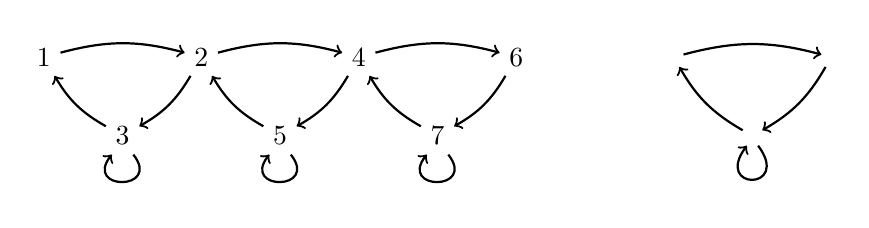
\begin{tikzpicture}
\node (1) at (0,1){1};
\node (2) at (2,1){2};
\node (3) at (1,0){3};
\node (4) at (4,1){4};
\node (5) at (3,0){5};
\node (6) at (6,1){6};
\node (7) at (5,0){7};
\node (...) at (7,1){};
\node (n3) at (8,1){};
\node (n1) at (10,1){};
\node (n) at (9,0){};
\draw[->,thick] (3.-60) .. controls (1.5,-0.7) and (0.5,-0.7) .. (3.-120);
\node at (1,-0.7){{\scriptsize}};
\draw[->,thick] (5.-60) .. controls (3.5,-0.7) and (2.5,-0.7) .. (5.-120);
\node at (3,-0.7){{\scriptsize}};
\draw[->,thick] (7.-60) .. controls (5.5,-0.7) and (4.5,-0.7) .. (7.-120);
\node at (5,-0.7){{\scriptsize}};
\draw[->,thick] (n.-60) .. controls (9.5,-0.7) and (8.5,-0.7) .. (n.-120);
\node at (9,-0.7){{\scriptsize}};
\path[->,thick,bend left=15]
(1) edge node[above=-0.5mm] {{\small }} (2)
(2) edge node[near start,below=0.2mm] {{\scriptsize }} (3)
(3) edge node[near end,below=0.2mm] {{\scriptsize }} (1)
(2) edge node[above=-0.5mm] {{\scriptsize }} (4)
(4) edge node[near start,below=0.2mm] {{\scriptsize }} (5)
(5) edge node[near end,below=0.2mm] {{\scriptsize }} (2)
(4) edge node[above=-0.5mm] {{\scriptsize }} (6)
(6) edge node[near start,below=0.2mm] {{\scriptsize }} (7)
(7) edge node[near end,below=0.2mm] {{\scriptsize }} (4)
(n3) edge node[above=-0.5mm] {{\scriptsize }} (n1)
(n1) edge node[near start,below=0.2mm] {{\scriptsize }} (n)
(n)  edge node[near end,below=0.2mm] {{\scriptsize }} (n3)
;
\end{tikzpicture}
\end{center}}
\end{example}

\begin{remark}\label{rem:upperbound}
{\em Theorems~\ref{newrule1} and \ref{renewrule1} are already relevant compared to the upper bounds  and . Indeed, if  is signed digraph described above,  then , thus the first upper-bound is exponential with , and  so the second upper bound is at least  by the Gilbert bound, and is also exponential with . However, as explained above,  satisfies the conditions of Theorems~\ref{newrule1} and \ref{renewrule1}, which give an upper bound equal to one only.}
\end{remark}

\begin{example}\label{ex2}
{\em Suppose that  is the signed digraph described below. Each negative cycle  is of length three and contains a vertex  with a positive loop. The arc  of  then satisfies the condition of Theorem \ref{newrule2}. Thus  has at least one fixed point.
\begin{center}
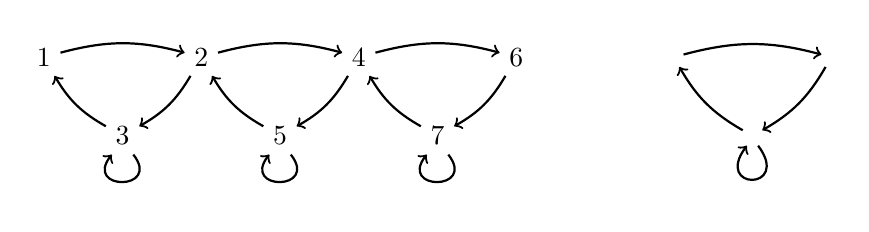
\begin{tikzpicture}
\node (1) at (0,1){1};
\node (2) at (2,1){2};
\node (3) at (1,0){3};
\node (4) at (4,1){4};
\node (5) at (3,0){5};
\node (6) at (6,1){6};
\node (7) at (5,0){7};
\node (...) at (7,1){};
\node (n3) at (8,1){};
\node (n1) at (10,1){};
\node (n) at (9,0){};
\draw[->,thick] (3.-60) .. controls (1.5,-0.7) and (0.5,-0.7) .. (3.-120);
\node at (1,-0.75){{\scriptsize}};
\draw[->,thick] (5.-60) .. controls (3.5,-0.7) and (2.5,-0.7) .. (5.-120);
\node at (3,-0.75){{\scriptsize}};
\draw[->,thick] (7.-60) .. controls (5.5,-0.7) and (4.5,-0.7) .. (7.-120);
\node at (5,-0.75){{\scriptsize}};
\draw[->,thick] (n.-60) .. controls (9.5,-0.7) and (8.5,-0.7) .. (n.-120);
\node at (9,-0.75){{\scriptsize}};
\path[->,thick,bend left=15]
(1) edge node[above=-0.5mm] {{\small }} (2)
(2) edge node[near start,below=0.2mm] {{\scriptsize }} (3)
(3) edge node[near end,below=0.2mm] {{\scriptsize }} (1)
(2) edge node[above=-0.5mm] {{\scriptsize }} (4)
(4) edge node[near start,below=0.2mm] {{\scriptsize }} (5)
(5) edge node[near end,below=0.2mm] {{\scriptsize }} (2)
(4) edge node[above=-0.5mm] {{\scriptsize }} (6)
(6) edge node[near start,below=0.2mm] {{\scriptsize }} (7)
(7) edge node[near end,below=0.2mm] {{\scriptsize }} (4)
(n3) edge node[above=-0.5mm] {{\scriptsize }} (n1)
(n1) edge node[near start,below=0.2mm] {{\scriptsize }} (n)
(n)  edge node[near end,below=0.2mm] {{\scriptsize }} (n3)
;
\end{tikzpicture}
\end{center}}
\end{example}

From a technical point of view, proofs are mainly based on refinements of Aracena's arguments. The innovation principally relies in the nature of the statements, which generalize previous results by taking into account both kinds of cycles simultaneously, and only use information on . For uniqueness results, we will prove a theorem that generalizes Theorem~\ref{rule1} and that directly implies Theorems~\ref{newrule1}, \ref{renewrule1} as well as upper bounds that only depend on  and that improve the two upper-bounds discussed above. 

\medskip
Let us say that a positive (resp. negative) arc of  from  to  is {\bf canalized} by  if there exists  such that  for all  with  (resp. ). The proofs reveal interesting properties on networks without canalized arc. In particular, using mainly graph theoretic arguments, we will prove the following theorem, established by Aracena under the hypothesis that  is strongly connected and has no negative cycle \cite[Theorem 6]{A08}. 

\begin{theorem}\label{strong}
If  is strongly connected, has a unique negative cycle and at least one positive cycle, and if  canalizes no arc that belongs to the negative cycle, then  has two fixed points with Hamming distance . 
\end{theorem}

Let us mention the few other theoretical works we know that consider connections between positive and negative cycles in Boolean networks. They differ from the present work by the hypothesis made on . In \cite{DNS12} and \cite{MNR14} is given a comprehensive analysis of the synchronous and asynchronous dynamics of Boolean networks whose interaction graph  consists of two cycles that share exactly one vertex ( is then a so-called double-cycle). Both in the synchronous and asynchronous case, the dynamics is easier to understand when both cycles are positive than when the two cycles have different signs, and the most intriguing and difficult case occurs when both cycles are negative. Besides, \cite{DR12} proposes a study of the number of fixed points under the following hypothesis:  is strongly connected, has a vertex  meeting every cycle, and all the vertices  are of in-degree one (so  and  has thus at most two fixed points). The results of \cite{DR12} not contained in \cite{A08} are then essentially the following. Firstly, if  has a unique positive (resp. negative) cycle and at least one negative (resp. positive) cycle, then  has at most (resp. at least) one fixed point (this is an easy consequence of Theorems~\ref{newrule1} and \ref{newrule2}, as explained below, in Remarks \ref{rem:DR1} and \ref{rem:DR2}). Secondly, if  has at least two positive cycles and two negative cycles, then  may have zero, one or two fixed points. Other works based on simulations and considering connections between positive and negative cycles can be found in \cite{KC07,SVL08}. 

 
\medskip 
The paper is organized as follows. Preliminaries are given in Section~\ref{sec:preliminaries}. Uniqueness results and the resulting upper-bounds are given in Sections~\ref{sec:uniqueness} and \ref{sec:upperbound}. Existence results are given in Section~\ref{sec:existence}. Concluding remarks are given in Section~\ref{sec:conclusion}. 

\section{Preliminaries}\label{sec:preliminaries}


A signed digraph  has a vertex set  and an arc set . Each arc  has an initial vertex , a terminal vertex , a {\em sign} , and is written as . We also say that  is an arc from  to , that  is an {\em in-coming arc} of  of sign , and that  is an {\em in-neighbor} of  of sign . The {\em in-degree} of  is the number of in-coming arcs of . A {\em source} is a vertex of in-degree zero. The set of in-neighbors of  is denoted , and the set of in-neighbors of sign  is denoted . We say that  is {\em simple} if  and  are disjoint for every vertex . We abusively write  to mean that  is the {\em trivial graph} with  as unique vertex and no arc. If  is another signed digraph then  is the signed digraph with vertex set  and arc set . If  then  has vertex set  and arc set . 

\medskip
A {\em subgraph} of  is a signed digraph obtained from  by removing arcs or vertices (with the attached arcs). We write  to mean that  is a subgraph of . If  is a vertex or an arc, then  is the subgraph obtained from  by removing . The subgraph of  {\em induced} by a set of vertices , denoted , is the subgraph obtained from  by removing every vertex not in . We denote by  the subgraph obtained from  by removing every arc with a terminal vertex in . 

\medskip
Paths and cycles of  are always directed and regarded as simple subgraphs. The {\em sign} of a path or a cycle is the product of the signs of its arcs. Thus a path or a cycle is positive if and only if it contains an even number of negative arcs. A {\em strong component} (or component for short) of  is a maximal set of vertices  (with respect to the inclusion relation) such that  is strongly connected ({\em strong} for short). Such a component  is {\em trivial} if . If  has no arc from  to  then  is an {\em initial component}. If  has no arc from  to , then  is a {\em terminal component}. If  is a cycle and  then  is the path from  to  contained in  (with the convention that this path is the trivial path  if ). If  is a path and if  and  are vertices in  such that  does not appear before  in , then  is the path from  to  contained in .  

\medskip
In all the following,  always denotes an -component Boolean network, that is , and  always denotes its interaction graph, as defined in the introduction. The vertex set of  is thus . If  and  then  is the restriction of  to the components in . The {\em Hamming distance} between two points , denoted , is the number of  such that . We denote by  the point  that differs from  only in . We denote by  the point at Hamming distance  from~. 

\medskip
For all vertex  of , we define the partial order  on  as follows: for all , 

Note that if  then  for all . A very basic property is that  is non-decreasing with respect to the partial order . 

\begin{lemma}\label{local_lemma}
For all  and ,

\end{lemma}


\begin{proof}[{\bf Proof}]
Let  be the set of  such that . We prove the lemma by induction on the size of . If  is empty, then we clearly have  thus the lemma holds. For the induction step, suppose that  contains some vertex  and that . If , then  thus . We deduce that , since otherwise  and thus , a contradiction. Furthermore, , and since , by induction hypothesis, . Hence,  as required. If  the proof is similar.
\end{proof}

For all , we denote by  the subgraph of  with vertex set  that contains all the  arcs  of  with  and all the arcs  of  with . Hence, a path of  from  to  is positive if  and negative if . As a consequence, we have the following basic property, used several times below.

\begin{lemma}
For all , all the cycles of  are positive.
\end{lemma}

\section{Uniqueness results}\label{sec:uniqueness}


Uniqueness results are based on the following definition. An arc  in a positive cycle  is a {\bf special arc} of  if the following holds in  :
\begin{itemize}
\item[]  is not a source,
\item[]  is not contained in a positive cycle,
\item[] every path from a positive cycle or a source to  intersects .
\end{itemize} 

The main result of this section is the following generalization of Theorem~\ref{rule1}. 

\begin{theorem}\label{uniqueness}
If  and  are distinct fixed points of , then  has a positive cycle  with no special arc such that  for every vertex  in . 
\end{theorem}


The following lemma has been proved in \cite[Theorem 9]{A08} and already implies Theorem~\ref{rule1}. We include a short proof for completeness.  

\begin{lemma}\label{alphabeta_lemma}
Suppose that  and  are distinct fixed points of . Then  has a cycle  such that  for all vertex  in . 
\end{lemma}


\begin{proof}[{\bf Proof}]
Let  be the set of  such that . Suppose, for a contradiction, that  has a source, say . If , it means that  for all  and  for all . Since  for all , we deduce that  and thus . Since  we have  which is a contradiction since . If  we obtain a contradiction similarly. Hence,  has no source and thus contains at least one cycle. 
\end{proof}

\begin{lemma}\label{source_lemma}
If  then every source of  is a source of . 
\end{lemma}


\begin{proof}[{\bf Proof}]
Suppose that  is a source of . If  it means that  for all  and  for all . Hence, for all , we have  and thus . Since , we deduce that  for all . Thus  is constant and this is equivalent to say that  is a source of . If  the proof is similar.  
\end{proof}

\begin{lemma}\label{canalizing}
Let  be a positive cycle of  with a special arc . Let  be a fixed point of , and suppose that . Then  for all  such that . 
\end{lemma}


\begin{proof}[{\bf Proof}]
Let us prove that  is a source of . Suppose, for a contradiction, that this is not the case, and let  be a path of  from a source or a cycle of  to . By Lemma~\ref{source_lemma}, every source of  is a source of , and since every cycle of  is a positive cycle of , we deduce that  is a path from a source or a positive cycle of  to . We deduce from the definition of a special arc that  intersects . Let  be the last vertex of  that belongs to . Then  is a cycle of . Thus  is a positive cycle of  containing , and this contradicts the fact that  is a special arc. Thus  is indeed a source of . 

\medskip
Let  with . Suppose that . Since  is a source of , we have  for all  and  for all . Since , we deduce that  and thus . Since , we obtain , as required. If  the proof is similar.  
\end{proof}

\begin{proof}[{\bf Proof of Theorem~\ref{uniqueness}}]
Let  and  be distinct fixed points of , and let  be the set of  such that . By Lemma~\ref{alphabeta_lemma},  has a cycle . It is thus sufficient to prove that  has no special arc. Suppose, for a contradiction, that  has a special arc . By Lemma~\ref{canalizing}, 

Since , by applying the same lemma, we get 

Since  and  we deduce that, for all ,  if and only if . Hence,  only depends on , so  is the unique in-coming arc of  in . Thus  is a source of , and this contradicts the fact that  is a special arc. Thus  has no special arc. 
\end{proof}

Theorems~\ref{newrule1} and \ref{renewrule1} stated in the introduction are easy corollaries of Theorem~\ref{uniqueness}.

\begin{proof}[{\bf Proof of Theorems~\ref{newrule1} and  \ref{renewrule1}}] 
In Theorem~\ref{newrule1}, each positive cycle  has an arc  satisfying some conditions that trivially imply that  is a special arc of . In Theorem~\ref{renewrule1}, each positive cycle  has a vertex  satisfying some conditions that trivially imply that the arc  of  with terminal vertex  is a special arc of . Thus in both cases, every positive cycle has a special arc and, by Theorem~\ref{uniqueness},  has at most one fixed point. 
\end{proof}

\begin{remark}\label{rem:DR1}
{\em An easy corollary of Theorem~\ref{uniqueness} is the following: 
\begin{quote}
{\em If  is strong, has a unique positive cycle  and at least one negative cycle, then  has at most one fixed point} (since every arc  of  such that  is of in-degree at least two is then a special arc of ).
\end{quote}
This has been proved in \cite{DR12} under the additional assumptions that there exists a vertex  meeting every cycle and that all the vertices  have in-degree one.}
\end{remark}

\begin{remark}
{\em Aracena proved in \cite{A08} the following: 
\begin{quote}
{\em If  has a non-trivial initial component without negative cycle, then  has no fixed~point.} 
\end{quote}
This follows directly from Lemma~\ref{source_lemma}. Indeed, if  has a non-trivial component  and  then, by Lemma~\ref{source_lemma},  has no source and thus at least one cycle , which is a positive cycle of . Furthermore, if  canalizes no arc of , then we deduce from Lemma~\ref{canalizing} that  has no special arc. Hence, we get a weaker sufficient condition for the absence of fixed point (which however does not only depend on ):}
\begin{quote}
If  has a non-trivial component  in which every positive cycle has a special arc, and if  canalizes no arc that belong to a positive cycle of , then  has no fixed~point.
\end{quote}
\end{remark}

\begin{remark}
{\em The notion of special arc relies on connections between positive and negative cycles in the following sense:
\begin{quote}
{\em If  has a special arc, then either  intersects a negative cycle or  has a non-trivial initial component with only negative cycles} (and thus  has no fixed point by the theorem of Aracena mentioned just above). 
\end{quote}
Indeed, suppose that  has a special arc . Since  is not a source of ,  has an arc . If  and  are not in the same  component, then  has a path  from an initial component  to  without vertex in . Since  is a special arc of , we deduce that  is not a source and has no positive cycle. So  is a non-trivial initial component of  with only negative cycles. If  and  are in the same component, then  has a path  from  to , and thus  is a cycle of  containing . Thus  is negative (since  is special) and  intersects .}
\end{remark}

\section{Upper-bounds}\label{sec:upperbound}


Let  be the minimum size of a set of vertices  such that, in , every positive cycle has a special arc. Let  be the minimum length of a positive cycle of  without special arc (with the convention that  if such a cycle does not exist). Below, we prove that  and  are upper bounds one the number of fixed points of . Since we always have  and , these upper-bounds improve the upper bounds  and  mentioned in the introduction. Actually, the gap can be arbitrarily large since if  is as in Example \ref{ex1} then  and , so that , while both  and  are exponential with , as explained in Remark~\ref{rem:upperbound}. 

\begin{corollary}\label{newupperbound}
 has at most  fixed points. 
\end{corollary} 


\begin{proof}[{\bf Proof}]
If  and  are two distinct fixed points of  then  has a positive cycle without special arc such that  for every vertex  of  (Theorem \ref{uniqueness}). Thus  is at most the length of , which is at most the Hamming distance between  and . Thus  has indeed at most  fixed points. 

\medskip
Let us now prove that  has at most  fixed points. Let  be a set of vertices of size  such that, in , every positive cycle has a special arc. Let  be the set of fixed points of  and suppose, for a contradiction, that . Then the function from  to  that maps  on  is not an injection, thus there exists distinct  such that . Let  be the -component network defined by  for every  and  for every . Then  and  are fixed points of  and thus, by Theorem  \ref{uniqueness}, the interaction graph of , which is precisely , has a positive cycle without special arc, a contradiction. Thus  as required. 
\end{proof}


\section{Existence results}\label{sec:existence}


We define a {\bf two-coloring} of  as a point  such that . In other words, regarding  as the color of vertex ,  is a two-coloring if all the negative arcs link vertices with the distinct colors, and all the positive arcs link vertices with the same color. If  has only negative arcs, we then recover the usual notion of (proper) two-coloring for unsigned graphs. Obviously,  is a two-coloring if and only if  is a two-coloring. 

\medskip
We denote by  the signed digraph obtained from  by adding an arc  for every arc  of . Hence,  can be regarded as the symmetric (or undirected) version of . A well known theorem of Cartwright and Harary \cite{CH56} asserts the following: 

\begin{theorem}\label{thm_Harary}
 has no negative cycle if and only if  has a two-coloring.
\end{theorem}

We will also use the following easy observation on the negative cycles of  and . 

\begin{lemma}\label{lem_GG*}
If  is strong, then  has a negative cycle if and only if  has a negative cycle.
\end{lemma}

Below are two easy applications of the fact that  is non-decreasing with .

\begin{lemma}\label{lem_ex_1}
Let  be a vertex of  of in-degree at least one and . If all the in-coming arcs of  are in  then . 
\end{lemma}


\begin{proof}[{\bf Proof}]
Suppose that all the in-coming arcs of  are in . If , then  for all  and  for all . Hence, for all , we have  and thus . We deduce that if , then  for all . But then  is a constant and this is equivalent to say that  is a source of , a contradiction. Therefore  as required. If  the proof is similar. 
\end{proof}

\begin{lemma}\label{lem_ex_2}
Let  be an arc of , and let  such that . Suppose that all the in-coming arcs of  distinct from  are in . Then  for all  such that . Furthermore,  if and only if . 
\end{lemma}


\begin{proof}[{\bf Proof}]
If , then  for all  and  for all . Hence, for all  such that , we have  and thus . Therefore,  as required. If  the proof is similar. Furthermore,  is not in , since otherwise  by Lemma \ref{lem_ex_1}. Thus  if  and  otherwise. 
\end{proof}

We are now in position to prove Theorem~\ref{newrule2}, that we restate from the introduction. 

\setcounter{theorem}{4}

\begin{theorem}
If every negative cycle of  has an arc  such that  has a non-trivial initial strong component containing  and only positive cycles, then  has at least one fixed point.
\end{theorem}


\begin{proof}[{\bf Proof}]
We proceed by induction on the number of negative cycles. If  has no negative cycle, then  has at least one fixed point by Theorem \ref{rule2}. So suppose that  has at least one negative cycle  and satisfies the condition of the theorem. By hypothesis,  has an arc  such that  has a non-trivial initial component  containing  and only positive cycles. Suppose that  is maximal in the following sense: for every arc  that belongs to a negative cycle and such that  has a non-trivial initial component  containing  and only positive cycles,  is not a strict subset of . 

\medskip
Let us prove that 
Let  be a negative cycle of  and let  be an arc of  such that  has a non-trivial initial component  containing  and only positive cycles. It is sufficient to prove that  is an initial component of . Since  is strong and  (because  and  are disjoint),  is strong. Thus if , then  is strong, and since  is an initial component of  we deduce that . Since , this contradicts the maximality of . Thus  and it is then straightforward to show that  is an initial component of . So  satisfies the condition of the theorem, as required. 

\medskip
Since  is strong and has no negative cycle, it follows that  has no negative cycle (by Lemma~\ref{lem_GG*}), and thus it has a two-coloring  (by Theorem~\ref{thm_Harary}). Consider the -component networks  and  defined as follows: 
8mm]
\left\{
\begin{array}{ll}
\hat f_w=\cst=1&\text{for all }w\in I\text{ with }\chi_w=0\\
\hat f_w=\cst=0&\text{for all }w\in I\text{ with }\chi_w=1\\
\hat f_w=f_w&\text{for all }w\notin I.\\
\end{array}
\right.
\end{array}
\label{eq:ab}
\forall w\neq v,\qquad f_w(x)=x_w\quad\text{and}\quad f_w(y)=y_w.

f_v(z)\neq x_v\text{ for all  such that }. 

f_v(z)\neq y_v\text{ for all  such that }. 
\label{eq:sign}
{\text{\em Each alternative path  from  to  has the same sign as .}}

C[u_2,v_2]\subseteq C[v_1,u_1].

H=P_1\cup C[v_1,u_2]\cup P_2\cup C[v_2,u_1]. 

s(W) =s(P_1)s(C[v_1,u_2])s(P_2)s(C[v_2,u_1])

s(W)=s(C[v_1,u_1])s(C[v_1,u_2])s(C[v_2,u_2])s(C[v_2,u_1]).

s(C[v_1,u_1])=s(C[v_1,u_2])s(C[u_2,v_2])s(C[v_2,u_1])

s(W) =s(C[u_2,v_2])s(C[v_2,u_2])s(C[v_1,u_2])^2s(C[v_2,u_1])^2
=s(C[u_2,v_2])s(C[v_2,u_2])=s(C).

H'= P_1'\cup C[v'_1,u_2]\cup P_2\cup C[v_2,u_1]

s(W') =s(P'_1)s(C[v'_1,u_2])s(P_2)s(C[v_2,u_1]).

s(W') =s(C[v'_1,u_1])s(C[v'_1,u_2])s(C[v_2,u_2])s(C[v_2,u_1]).

s(C[v'_1,u_1])=s(C[v'_1,u_2])s(C[u_2,v_2])s(C[v_2,u_1])

s(W') =s(C[u_2,v_2])s(C[v_2,u_2])s(C[v'_1,u_2])^2s(C[v_2,u_1])^2=s(C).

Hence,  is an negative closed walk, thus  has a negative cycle . Since  is arc-disjoint from , , a contradiction.
\end{proof}

\begin{proof}[{\bf Proof of Theorem \ref{strong}}]
Let  be the unique negative cycle of . Let  be the set of arcs of  that belong to no positive cycle, which is not empty by Lemma~\ref{graph}. Suppose that , and let  be the arc succeeding  in . If  is of in-degree one, then every cycle containing  contains also  and thus . Since some vertex of  is of in-degree at least two, we deduce that there exists an arc in , say ,  such that  is of in-degree at least two. 

\medskip
Let  be an enumeration of the components of  in the topological order (that is, in such a way that for all ,  has no arc from  to ). Since  is strong,  (resp. ) is the unique initial (resp. terminal) component of , and  (resp. ). Suppose that there exists two distinct arcs leaving a component , . Then  has two distinct paths from  to , and this contradict that fact that  is the unique cycle containing~. We deduce that, for each , there is a unique arc, say , leaving the component . Then , since otherwise there is an initial component distinct from . Since every component  has no negative cycle, we deduce that  has no negative cycle, and so  has a two-coloring . 

\medskip
Since  is of in-degree at least two in ,  has no source, and thus we deduce from Lemma~\ref{lem_ex_1} that  for all . From Lemma~\ref{lem_ex_2}, if  then  canalizes , a contradiction. Thus  and we prove with similar arguments that . 
\end{proof}

\section{Concluding remarks}\label{sec:conclusion}


We have established new sufficient conditions, expressed on  only, for the uniqueness (resp. existence) of a fixed point of . In order to know if it is reasonable to think about a characterization, it could be interesting to study the complexity of the following decision problem: {\em Given an signed digraph , is it true that all the Boolean networks with  as interaction graph have at most (resp. at least) one fixed point?}

\medskip
We have established an upper-bound on the number of fixed points, namely , that improve the classic bound . This new bound raise some questions. Let  be the maximal number of fixed points in a Boolean network with  as interaction graph. The signed digraph in Example \ref{ex1} shows that  does not necessarily increase with . We can ask if the situation is identical with : {\em Does  necessarily increase with ? In other words, is there exists an unbounded function , independent of , such that ?} 

\medskip
Let  be the digraph with vertex set  and with an arc from  to  if there exists  such that  and . This digraph  is usually called the {\em asynchronous state graph} of , and is a classical model for the dynamic of gene network \cite{TA90,TK01}. The terminal components of  are then regarded as the attractors of the system and called {\em attractors} of . Hence, fixed points are attractors of cardinality one. Attractors of size at least two are called {\em cyclic attractors}. It is known that the upper-bounds  and  are actually upper-bounds one the number of attractors in  \cite{R09}. {\em Is it also the case with the new bounds  and ?} Besides, it is known that if  has no negative cycle, then  has no cyclic attractor (and this trivially implies that  has a fixed point) \cite{R10}. {\em Is the weaker condition in Theorem~\ref{newrule2} also sufficient for the absence of cyclic attractors in ?} 


\medskip
In the proof of Theorem~\ref{strong}, we show that a signed digraph with a unique negative cycle is very-well structured and, in particular, is not -arc-strongly connected. Continuing this direction, it could be interesting to study the structure of signed digraphs in which all the negative cycles are vertex disjoint, in order to obtain a sufficient condition for the presence of a fixed point with the spirit of the condition in Theorem~\ref{renewrule1}. 

\paragraph{Acknowledgment} I wish to thank Emmanuelle Seguin and Isabelle Soubeyran for stimulating discussions. 

\bibliographystyle{plain}
\bibliography{bib}

\end{document}
